\section{Introduzione alla Data Augmentation}

\subsection{Definizione}
La data augmentation è una tecnica utilizzata nel campo del machine learning per incrementare la quantità e la varietà dei dati di addestramento a disposizione. 

\begin{figure}[ht]
    \centering
    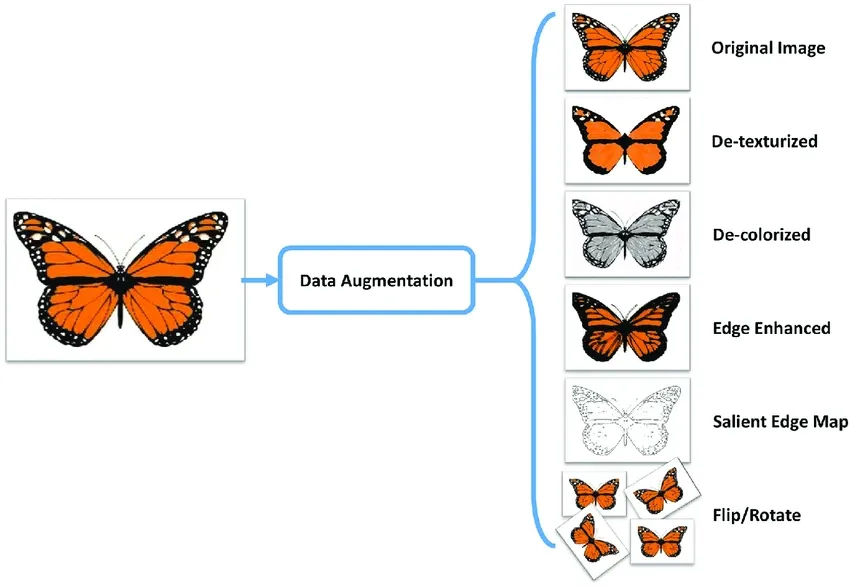
\includegraphics[width=0.7\textwidth]{files/capitoli/3-data-augmentation/assets/augmentation-example.png}
    \caption{\label{fig:augmentation-example}Esempi di Augementation su un'immagine\cite{33}}
\end{figure}

\newpage

Questa tecnica consiste nel generare nuovi dati a partire da quelli esistenti, applicando una serie di trasformazioni come rotazioni, traslazioni, modifiche di colore, aggiunta di rumore, e molte altre. Si può quindi definire come un insieme di operazioni che modificano i dati originali in modo da creare nuove versioni, pur mantenendo inalterata l'informazione essenziale contenuta nei dati stessi.

\subsection{Scopo}
L'obiettivo principale della data augmentation è quello di migliorare la generalizzazione dei modelli di machine learning, ovvero la capacità del modello di performare bene su dati mai visti prima. Questo viene ottenuto in vari modi:
\begin{itemize}
  \item \textbf{Aumento della Varietà dei Dati}: aggiungendo varianti dei dati esistenti, si espande il dataset senza la necessità di raccogliere nuovi dati. Questo è particolarmente utile quando i dati disponibili sono limitati o costosi da ottenere.
  \item \textbf{Riduzione dell'Overfitting}: creando una maggiore diversità nel dataset, si riduce il rischio che il modello impari a memorizzare dettagli specifici dei dati di addestramento piuttosto che generalizzare dai pattern sottostanti (fenomeno dell'overfitting), e si costringe quindi il modello a imparare caratteristiche più generali e robuste.
  \item \textbf{Bilanciamento dei Dataset}: nei casi in cui alcuni gruppi di dati sono sottorappresentati (ad esempio, minoranze di classe in un problema di classificazione), la data augmentation può essere utilizzata per creare più esempi di queste classi minoritarie, aiutando a bilanciare il dataset e migliorare le prestazioni del modello su tutte le classi.
\end{itemize}

\newpage
